% !TeX root = ../build/main.tex

\paragraph{Vision and background.}

Voĉdoni, meaning “to give voice” in Esperanto, embodies our mission to empower civil society from the grassroots level. We aim to build essential primitives and tools that enable any collective—from small groups to millions of citizens—to be heard, regardless of their circumstances or available resources. Our philosophy envisions voting beyond traditional nation-state elections; we see it as a collective signaling mechanism with cryptographic guarantees of integrity and outcome. To address the challenge, we developed a end-to-end verifiable and anonymous voting system designed to work on any device, including smartphones. We also successfuly deployed an infrastructure that maximizes resilience, neutrality, and transparency.

In 2018, when Vocdoni began, zkSNARKs was just an emerging technology. We chose to base our solution on a customized Byzantine fault tolerant layer-1 (L1) blockchain called Vochain. This allowed us to achieve scalability (approximately 700 transactions per second), to leverage advanced cryptographic tools that are prohibitively expensive on EVM-based blockchains, and enable users to send voting transactions without costs. This experience has provided us with invaluable insights that have enabled us to overcome technical and operational challenges. Although this solution has effectively met user requirements and demonstrated its viability, further development is essential for its widespread adoption as a universal voting protocol.

\Davinci represents the evolution of the Vocdoni voting protocol. It integrates smart contracts for orchestration, a zkSNARK-based state machine for verifying and accumulating votes, and a decentralized data availability layer to ensure censorship resistance.

\paragraph{Design principles.}

To build the \davinci stack, we adhere to the following design principles:

\begin{enumerate}
	\item \textbf{Cryptography as the source of truth}: we rely exclusively on cryptographic proofs to ensure the integrity and security of the voting process. By trusting only in cryptography, we eliminate the need for centralized authorities, making the system inherently secure and transparent.
	
	\item \textbf{Trustlessness}: our system operates without requiring trust in any single party. Through cryptographic protocols and decentralized infrastructure, we ensure system integrity and prevent compromise from any malicious actor.
	
	\item \textbf{End-to-end verifiability}: every voter can verify their ballot from casting to result computation (individual verifiability). Additionally, any third party can audit the election data to confirm results (universal verifiability) and verify that each vote comes from a uniquely registered voter (eligibility verifiability). Transparent cryptographic mechanisms make this possible.
	
	\item \textbf{Composability}: the system is modular, consisting of interchangeable components that can be rearranged or integrated with external systems via adaptable interfaces. This allows for redundancy, flexibility, and seamless integration with third-party applications, exemplified by our voting-as-a-service APIs.
	
	\item \textbf{Accessibility}: Vocdoni’s voting platform (App) is open source, universally available and user-friendly. The interface is intuitive for all users, including those less familiar with technology, and accommodates voters that use assistive technologies like screen readers.
	
	\item \textbf{Open source}: by releasing our code openly, we invite anyone to audit and contribute, enhancing security and fostering community engagement. Transparency prevents security through obscurity and accelerates innovation.
	
	\item \textbf{Resilience}: we design for robustness against hardware failures, network outages, and censorship. Infrastructure decentralization and distributed ownership enhance system availability and resistance to attacks.
	
	\item \textbf{Scalability}: our solution processes votes at high throughput, exceeding current requirements to accommodate future growth. The decentralized infrastructure scales organically as usage increases, ensuring consistent performance.
	
	\item \textbf{Receipt-freeness}: to mitigate risks of collusion, coercion, and vote-buying, the system enables voters to verify their votes without being able to prove to others how they voted, thus reducing incentives for coercion and bribery. Additionally, voters are allowed to overwrite their votes while maintaining secrecy.
	
	\item \textbf{Automation}: we minimize human intervention through smart contracts and cryptographic protocols, reducing costs and human error. Automation ensures consistent operation and frees resources for voter support and auditing.
\end{enumerate}

\paragraph{Components overview.}

Below, we detail the components of the architecture that collectively support the operation and management of the voting system.

\begin{figure}[h]
	\centerline{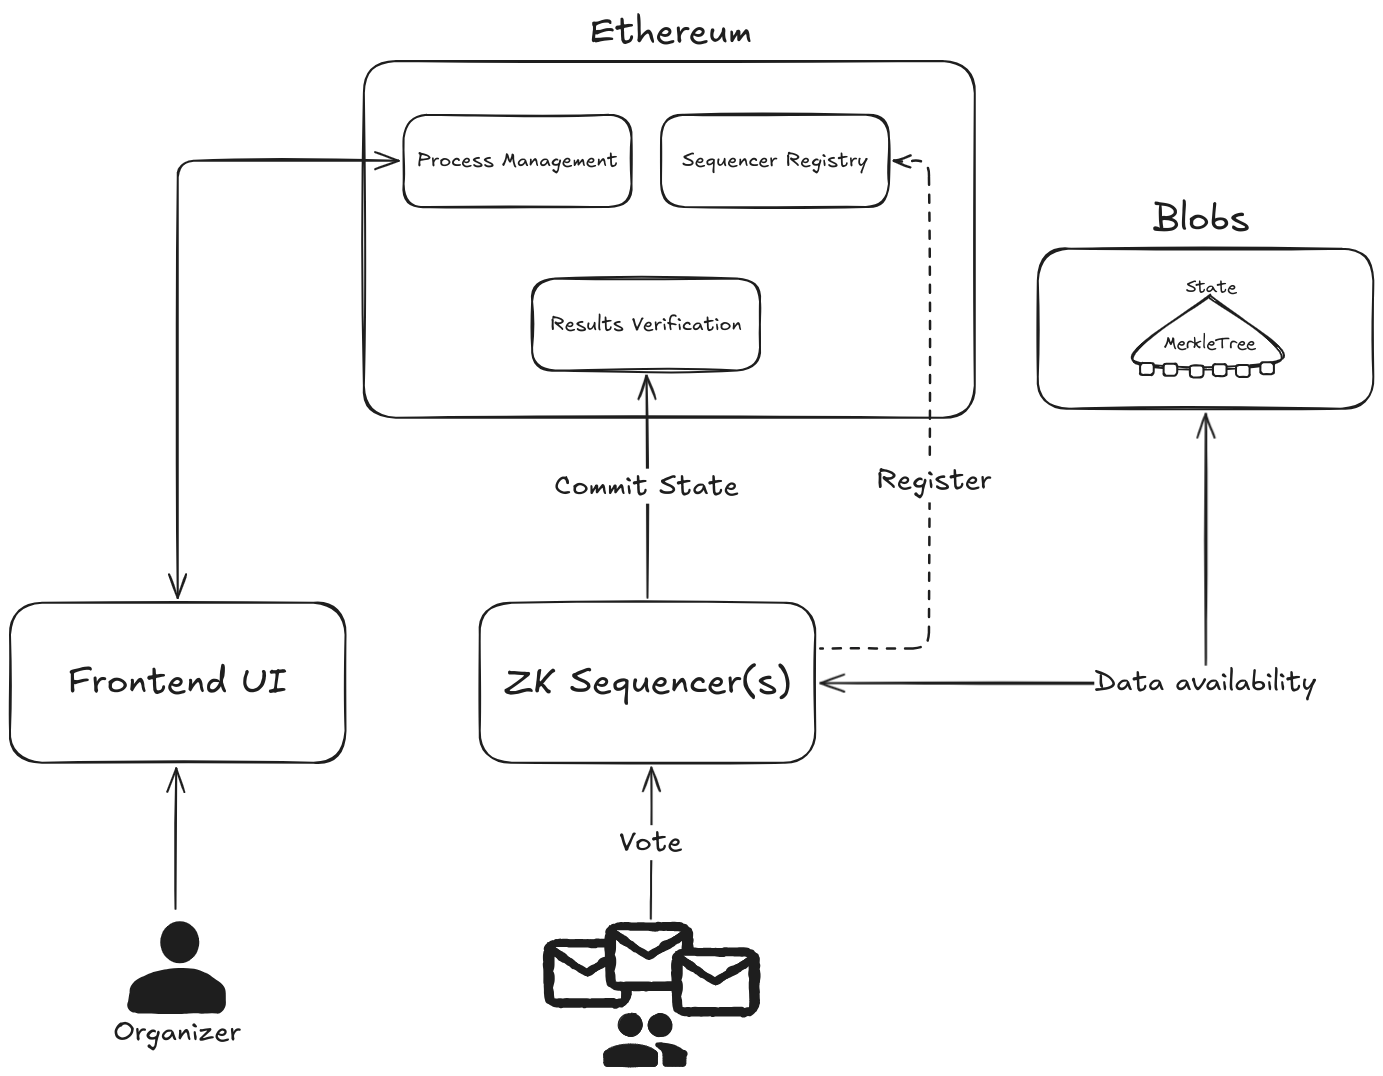
\includegraphics[width=300pt,draft=false]{\figs/architecture.png}}
	\caption{Caption.}
	\label{fig:circuit-inputs}
\end{figure}

\begin{enumerate}
	\item \textbf{Ethereum}. An Ethereum compatible network is used as the source of truth for the voting system. By leveraging an EVM blockchain, the process management ensures that all transitions are immutable and verifiable by all participants. To this end, we implement several smart contracts.
		\begin{itemize}
			\item \textbf{Process management}: Responsible for the lifecycle management of voting processes. It includes the initiation, monitoring, execution, and closure of voting events.
			\item \textbf{Results verification}: For each voting process, this smart contract maintains the integrity of the cast votes and process lifecycle. It verifies that each state transition committed by a ZK sequencer adheres to the predefined rules.			
			\item \textbf{Sequencer registry}: This smart contract keeps track of the existing available sequencers, stores the collateral to ensure good behavior, and it's used to coordinate the distributed key generation when a new Process is created.
		\end{itemize}
	\item \textbf{Sequencer}. The Sequencer is a specialized component designed to handle the voting process using zero-knowledge proof mechanisms. It ensures that all transactions related to this process are validated and sequenced. The Sequencers periodically commit the state of the voting process to Ethereum.
	\item \textbf{Frontend user interface}. The user interface serves as the primary interaction layer for voters and organizers. It provides tools and functionalities needed by organizers to set up, manage, and oversee elections. This interface simplifies the complexities involved in managing a decentralized vote.
	\item \textbf{Data availability}. For each voting process, the system needs to keep track of the current State Merkle Tree, which contains all information of such processes. A public data availability layer, ensures that all state transitions are available and verifiable and allows the participation of multiple sequencers within the same voting process.
\end{enumerate}
